\section{Auswertung}
In Tabelle \ref{tab:Messwerte} sind die genommenen Messwerte für die Auf- und Abstiegszeiten
$t_{\text{auf}}$ und $t_{\text{ab}}$ der 16 Tröpfchen bei verschieden Spannungen $U$ und Temperaturen $T$,
die durch eine Widerstandsmessung $R$ eines Thermowiderstands gemessen worden ist. $t_0$ ist die
Fallzeit des Tröpfchens bei nicht angelegter Spannung $U$. Die Zeit ist auf einer Distanz von $s=\qty{5e-4}{\meter}$
gemessen worden. Nun werden die Auf- und Abstiegszeiten über die 3 genommenen Messwerte gemittelt. Der Mittelwert der Zeiten ergibt sich durch
\begin{equation}\label{eq:mean}
    \overline{t_\text{x}}=\frac{1}{3}\sum_{i=1}^3t_\text{xi}\,
\end{equation}
und die Standardabweichung des Mittelwerts durch
\begin{equation}\label{eq:std}
    \Delta{t_\text{x}}=\sqrt{\frac{1}{3(3-1)}\sum_{i=1}^3\left(t_\text{xi}-\overline{t_\text{x}}\right)}\,.
\end{equation}
Die entsprechenden Werte sind in Tabelle \ref{tab:Mittel} zu finden.
Aus den gemittelten Zeiten und der Fallstrecke $s$ lassen sich nun die mitteleren Geschwindigkeiten
durch 
\begin{equation}\label{eq:v}
    \overline{v}=\frac{s}{\overline{t}}
\end{equation}
berechnen, wobei der Fehler sich durch 
\begin{equation}\label{eq:dv}
    \Delta{v}=\overline{v}\cdot \frac{\Delta t}{\overline{t}}
\end{equation}
ergibt. Dabei resultieren die Abweichungen im Ort, also die Ungenauigkeit das Intervall von $s$ genau einzuhalten, ebenfalls in der Ungenauigkeit in der Zeit. Daher beschreibt die statistisch ermittelte
Abweichung in der Zeit auch eine generelle Schwankung im Ort. Eine reine Ortsmessung würde einem Fehler
von $s=1e-4$ genügen. Die gemittelten Geschwindigkeiten finden sich ebenfalls in Tabelle \ref{tab:Mittel}. 
\label{sec:Auswertung}
\begin{table}[H]
    \centering
    \caption{Messwerte für alle 16 Tropfen.}
    \label{tab:Messwerte}
    \begin{tabular}{S[table-format=2] S[table-format=1.2] S[table-format=3] S[table-format=2.2]S[table-format=1.2]S[table-format=1.2]S[table-format=1.2]S[table-format=1.2]S[table-format=1.2]S[table-format=1.2]}
        \toprule
        {Tröpfchen}&{R/$\unit{\ohm}$}&{$U/\unit{\volt}$}&{$t_0/\unit{\s}$}&{$t_{auf1}/\unit{\s}$}&{$t_{auf2}/\unit{\s}$}&{$t_{auf3}/\unit{\s}$}&{$t_{ab1}/\unit{\s}$}&{$t_{ab2}/\unit{\s}$}&{$t_{ab3}/\unit{\s}$}\\
        \midrule
        1 & 2,27 & 244 & 35,73 & 2,59 & 6,49 & 5,71 & 3,46 & 2,47 & 4,05 \\
        2 & 2,25 & 244 & 47,47 & 9,26 & 8,65 & 4,07 & 6,97 & 6,08 & 7,04 \\
        3 & 2,25 & 244 & 56,78 & 2,94 & 4,85 & 2,16 & 2,29 & 3,14 & 1,37 \\
        4 & 2,24 & 244 & 40,59 & 2,85 & 2,89 & 8,19 & 2,37 & 2,70 & 6,61 \\
        5 & 2,22 & 200 & 44,13 & 3,25 & 3,55 & 1,52 & 3,00 & 2,90 & 2,77 \\
        6 & 2,22 & 200 & 46,78 & 5,04 & 5,57 & 2,40 & 3,29 & 5,51 & 3,35 \\
        7 & 2,22 & 200 & 56,72 & 4,34 & 2,36 & 1,97 & 1,84 & 1,45 & 4,53 \\
        8 & 2,22 & 200 & 49,38 & 4,66 & 2,63 & 2,84 & 3,92 & 3,47 & 2,50 \\
        9 & 2,22 & 295 & 44,94 & 1,40 & 1,91 & 1,07 & 0,80 & 1,07 & 1,45 \\
        10 & 2,22 & 295 & 47,84 & 1,58 & 3,74 & 3,08 & 3,41 & 2,83 & 2,70 \\
        11 & 2,22 & 295 & 8,44 & 2,51 & 1,98 & 5,50 & 1,26 & 1,19 & 2,11 \\
        12 & 2,22 & 295 & 44,30 & 1,26 & 1,64 & 2,12 & 1,13 & 1,98 & 2,04 \\
        13 & 2,22 & 225 & 30,60 & 6,87 & 2,82 & 3,35 & 3,22 & 3,22 & 3,99 \\
        14 & 2,20 & 225 & 38,49 & 2,95 & 2,50 & 3,48 & 2,58 & 2,57 & 2,90 \\
        15 & 2,20 & 225 & 74,60 & 0,99 & 1,60 & 1,65 & 1,60 & 5,71 & 1,65 \\
        16 & 2,17 & 225 & 61,00 & 1,38 & 1,12 & 2,95 & 1,12 & 1,31 & 1,14 \\
        \bottomrule
    \end{tabular}
  \end{table}

  \begin{table}[H]
    \centering
    \caption{Gemittelte Auf- und Abstiegszeiten und Geschwindigkeiten}
    \label{tab:Mittel}
    \begin{tabular}{c c c c c c}
        \toprule
        {$t_{auf}/\unit{\s}$}&{$t_{ab}/\unit{\s}$}&{$v_{auf}/10^{-5}\unit{\meter\per\s}$}&{$v_{ab}/10^{-5}\unit{\meter\per\s}$}&{$v_{0}/10^{-6}\unit{\meter\per\s}$}&{$\eta_0/10^{-5}\unit{\newton\second\per\meter\squared}$}\\
        \midrule
        $4,93 \pm 1,19$ & $3,33 \pm 0,46$ & $10,14 \pm 2,45$ & $15,03 \pm 2,08$ & $13,99$ & $1,827$ \\
        $7,33 \pm 1,64$ & $6,70 \pm 0,31$ & $6,82 \pm 1,53$ & $7,47 \pm 0,34$ & $10,53$ & $1,831$ \\
        $3,32 \pm 0,80$ & $2,27 \pm 0,51$ & $15,08 \pm 3,63$ & $22,06 \pm 4,97$ & $8,81$ & $1,831$ \\
        $4,64 \pm 1,77$ & $3,89 \pm 1,36$ & $10,77 \pm 4,11$ & $12,84 \pm 4,49$ & $12,32$ & $1,831$ \\
        $2,77 \pm 0,63$ & $2,89 \pm 0,07$ & $18,03 \pm 4,11$ & $17,30 \pm 0,40$ & $11,33$ & $1,831$ \\
        $4,34 \pm 0,98$ & $4,05 \pm 0,73$ & $11,53 \pm 2,61$ & $12,35 \pm 2,23$ & $10,69$ & $1,831$ \\
        $2,89 \pm 0,73$ & $2,61 \pm 0,97$ & $17,30 \pm 4,39$ & $19,18 \pm 7,12$ & $8,82$ & $1,831$ \\
        $3,38 \pm 0,64$ & $3,30 \pm 0,42$ & $14,81 \pm 2,83$ & $15,17 \pm 1,93$ & $10,13$ & $1,831$ \\
        $1,46 \pm 0,24$ & $1,11 \pm 0,19$ & $34,25 \pm 5,73$ & $45,18 \pm 7,70$ & $11,13$ & $1,831$ \\
        $2,80 \pm 0,64$ & $2,98 \pm 0,22$ & $17,86 \pm 4,08$ & $16,78 \pm 1,23$ & $10,45$ & $1,831$ \\
        $3,33 \pm 1,10$ & $1,52 \pm 0,30$ & $15,02 \pm 4,94$ & $32,89 \pm 6,40$ & $59,24$ & $1,831$ \\
        $1,67 \pm 0,25$ & $1,72 \pm 0,29$ & $29,88 \pm 4,44$ & $29,13 \pm 4,99$ & $11,29$ & $1,831$ \\
        $4,35 \pm 1,27$ & $3,48 \pm 0,26$ & $11,50 \pm 3,36$ & $14,38 \pm 1,06$ & $16,34$ & $1,831$ \\
        $2,98 \pm 0,28$ & $2,68 \pm 0,11$ & $16,80 \pm 1,60$ & $18,63 \pm 0,75$ & $12,99$ & $1,831$ \\
        $1,41 \pm 0,21$ & $2,99 \pm 1,36$ & $35,38 \pm 5,31$ & $16,74 \pm 7,63$ & $6,70$ & $1,831$ \\
        $1,82 \pm 0,57$ & $1,19 \pm 0,06$ & $27,52 \pm 8,66$ & $42,02 \pm 2,13$ & $8,20$ & $1,833$ \\

        \bottomrule
    \end{tabular}
  \end{table}
\noindent Bevor nun die Ladungsmengen der Tröpfchen bestimmt wird, soll nun zuerst die Viskosität der Luft bestimmt werden.
Nach Tabelle \ref{fig:Wid} sollen nun den Widerständen $R$ eine Temperatur zugeordnet werden. Demnach entspricht der
Widerstand von Tröpfchen 1 ungefähr einer Temperatur von $21°\symup{C}$ und das letzte Tröpfchen einer Temperatur von $20°\symup{C}$. Den anderen Tröpfchen
liegen liegen vom Widerstandswert ziemlich dazwischen. Deswegen sind diesen Tröpfchen eine Temperatur von $21,5°\symup{C}$ zugeordnet worden.
In Abbildung \ref{fig:Vis} ist die Temperatur-Abhängigkeit zwischen Viskosität und Temperatur linear approximiert.
Es lässt sich erkennen, dass $T=16°\symup{C}$ einer Viskosität von $\eta=\qty{1.805e-5}{\newton\second\per\meter\squared}$
und $T=32°\symup{C}$ einer Viskosität von $\eta=\qty{1.881e-5}{\newton\second\per\meter\squared}$ entspricht.
Dadurch ergibt sich der lineare Zusammenhang zwischen Temperatur und Viskosität von
\begin{equation}
    \eta=(T-16°C)\cdot \qty{4.75e-8}{\newton\second\per\kelvin\meter\squared}+\qty{1.805e-5}{\newton\second\per\meter\squared}
\end{equation}
Die sich ergebenden Viskositäten sind in Tabelle \ref{tab:Mittel} zu sehen. Die Viskositäten müssten noch wegen der kleinen Abmessung
korrigiert werden. Diese Korrektur wird allerdings direkt auf die Ladung der Tröpfchen gemäß \eqref{eq:qkor}
angewendet. Nun werden die Differenz- und Summengeschwindigkeiten $v_\text{diff}=v_\text{ab}-v_\text{auf} $ und $v_\text{summ}=v_\text{ab}+v_\text{auf}$
berechnet. Die mögliche Abweichung ergibt sich bei beiden zu $\Delta v_\text{diff/summ}=\sqrt{\Delta v_\text{ab}^2+\Delta v_\text{auf}^2}$.
Die entsprechenden resultierenden Werte für die Tröpfchen sind in Tabelle \ref{tab:Ergebnis} zu sehen.
Nun sollen anhand von $v_\text{diff}$ einige Tropfen aussortiert werden. Dafür werden zunächst Kriterien angewendet.
Einmal soll $v_\text{diff}$ positiv sein. Da die fallenden Tröpfchen auf Grund der zusätzlich wirkenden Gravitationskraft schneller sein müssen.
Außerdem soll die Bedingung $2v_0=v_\text{diff}$. Diese Bedingung soll als erfüllt gelten, wenn 
$\left|2v_0-v_\text{diff}\right|<\Delta v_\text{diff}$ gilt. Auf Grund der sehr großen Abweichung schließt das nur 
die Tröpfchen 5,10,12,15 und 16 aus. Zur Bestimmung der Elementarladung wird daher noch ein anderes Auschlusskriterium von
Nöten sein.
\begin{figure}[H]
    \centering
    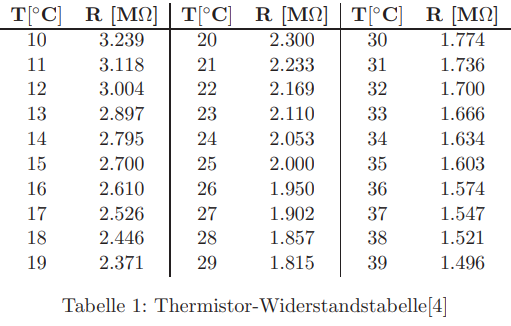
\includegraphics{content/Widerstand.png}
    \caption{Widerstandstabelle für Temperaturen}
    \label{fig:Wid}
  \end{figure}
  \begin{figure}[H]
    \centering
    \includegraphics{content/Viskosität.png}
    \caption{linearer Zusammenhang zwischen Viskosität und Temperatur}
    \label{fig:Vis}
  \end{figure}
Nun wird nach Gleichung \eqref{eq:q} die Ladung der Tropfen $q_0$ berechnet. Der Fehler ergibt sich durch
\begin{equation}
    \Delta q_0=\overline{q_0}\cdot \Delta v_\text{diff}\cdot \sqrt{\frac{1}{4v_\text{diff}^2}+\frac{1}{v_\text{summ}^2}}.
\end{equation}
Dabei ist der Plattenabstand der Kondensatoren $d=\qty{7.625e-3}{\meter}$, die Dichte von Öl 
$\rho_\text{öl}=\qty{886}{kilogram\per\meter\cubed}$ und $g$ die Erdbeschleunigung. Der Auftrieb in Form der Dichte der Luft
wird gegenüber der Dichte des Öls vernachlässigt.
Der Radius der Tropfen ergibt sich nach Gleichung \eqref{eq:r} und der Fehler durch
\begin{equation}
    \Delta r=\frac{\overline{r}}{2v_\text{diff}}\cdot \Delta v_\text{diff}.
\end{equation}
Die entsprechenden Werte für $r$ und $q_0$ sind in Tabelle \ref{tab:Ergebnis} abgebildet.
Die Ladungsmenge ist noch nicht vollständig korrekt, da die Viskosität noch durch den Cunningham-Korrekturterm
ergänzt werden muss. Das resultiert zu einer Korrektur der Ladung gemäß Gleichung \eqref{eq:qkor} zu
\begin{equation}
    \overline{q}=\overline{q_0}\cdot (1+\frac{B}{p\overline{r}})^{-3/2}.
\end{equation}
Dabei sind $B=\qty{6.71e-3}{\centi\meter}\cdot\text{torr}$ und $p=\qty{760}{}\text{torr}$, ein Atmosphärendruck.
Die Fehler pflanzen sich gemäß der Fehlerfortpflanzung durch
\begin{equation}
    \Delta{q}=\sqrt{(\frac{\overline{q}\Delta q}{\overline{q_0}})^2+(\frac{3B\overline{q_0}\Delta r}{2p*r^2})^2\cdot(1+\frac{B}{pr})}
\end{equation}
fort. Die korrigierten Ladungen $q$ sind ebenfalls in Tabelle \ref{tab:Ergebnis} eingetragen.
Ladung und Radius der einzelnen Tropfen sind inklusiver ihres Fehlers in Abbildung \ref{fig:Ladung} aufgetragen. Es lässt sich in diesem
Plot klar erkennen, dass die Tröpfchengröße direkt mir der Ladung korreliert, in dem Sinne, dass größere Tropfen mehr Ladung fassen.
\begin{table}[H]
    \centering
    \caption{Differenz und summierte Geschwindigkeit und Ladung und Radius der Tröpfchen}
    \label{tab:Ergebnis}
    \begin{tabular}{c c c c c }
        \toprule
        {$2v_0-v_{diff}/10^{-6}\unit{\meter\per\s}$}&{$v_{diff}/10^{-6}\unit{\meter\per\s}$}&{$q_0/10^{-19}\unit{\coulomb}$}&{$q_{\text{Tröpfchen}}/10^{-19}\unit{\coulomb}$}&{$r_{\text{Tröpfchen}}/10^{-7}\unit{\meter}$}\\
        \midrule
        $-20,89$ & $48,88 \pm 32,16$ & $6,52 \pm 2,30$ & $8,24 \pm 2,97$ & $4,81 \pm 1,58$ \\
        $14,65$ & $6,42 \pm 15,64$ & $1,34 \pm 1,64$ & $2,39 \pm 3,23$ & $1,74 \pm 2,13$ \\
        $-52,22$ & $69,83 \pm 61,59$ & $11,52 \pm 5,43$ & $14,05 \pm 6,72$ & $5,75 \pm 2,54$ \\
        $3,89$ & $20,74 \pm 60,90$ & $3,99 \pm 5,95$ & $5,64 \pm 8,79$ & $3,14 \pm 4,60$ \\
        $29,94$ & $-7,28 \pm 41,32$ & $4,32 \pm 12,27$ & $7,44 \pm 23,23$ & $1,86 \pm 5,27$ \\
        $13,22$ & $8,16 \pm 34,28$ & $3,09 \pm 6,50$ & $5,19 \pm 11,92$ & $1,97 \pm 4,13$ \\
        $-1,18$ & $18,81 \pm 83,70$ & $7,17 \pm 16,04$ & $10,28 \pm 24,14$ & $2,99 \pm 6,65$ \\
        $16,66$ & $3,59 \pm 34,21$ & $2,57 \pm 12,26$ & $5,32 \pm 29,21$ & $1,31 \pm 6,21$ \\
        $-87,09$ & $109,34 \pm 95,96$ & $25,51 \pm 11,61$ & $29,95 \pm 13,78$ & $7,20 \pm 3,16$ \\
        $31,69$ & $-10,79 \pm 42,57$ & $3,49 \pm 6,91$ & $5,54 \pm 11,77$ & $2,26 \pm 4,46$ \\
        $-60,31$ & $178,80 \pm 80,85$ & $19,68 \pm 5,55$ & $22,34 \pm 6,33$ & $9,21 \pm 2,08$ \\
        $30,12$ & $-7,54 \pm 66,78$ & $4,98 \pm 22,04$ & $8,51 \pm 41,31$ & $1,89 \pm 8,37$ \\
        $3,89$ & $28,79 \pm 35,27$ & $5,59 \pm 3,51$ & $7,53 \pm 4,89$ & $3,69 \pm 2,26$ \\
        $7,62$ & $18,36 \pm 17,67$ & $6,11 \pm 2,96$ & $8,80 \pm 4,47$ & $2,95 \pm 1,42$ \\
        $199,77$ & $-186,36 \pm 92,99$ & $28,65 \pm 8,79$ & $32,45 \pm 10,00$ & $9,40 \pm 2,35$ \\
        $-128,55$ & $144,94 \pm 89,18$ & $33,78 \pm 11,26$ & $38,86 \pm 13,05$ & $8,30 \pm 2,55$ \\
        \bottomrule
    \end{tabular}
\end{table}

\begin{figure}[H]
    \centering
    \includegraphics{build/Ladungen.pdf}
    \caption{Auftragen der Ladung gegen den Radius aller Tröpfchen}
    \label{fig:Ladung}
  \end{figure}

  \noindent Nun soll die Elementarladung als gemeinsamer Teiler der Ladungen der Tröpfchen bestimmt werden.
  Dabei werden nun allerdings zunächst noch zusätzlich alle Tropfen ausgeschlossen, wo die Unsicherheit der Ladungsmenge 
  größer als die Ladung selbst ist, ausgeschlossen, da die Ladungsmenge dieser Tropfen praktisch weiterhin unbekannt ist.
  Damit bleiben Tropfen 1,3,9,11,13 und 14 zur Analyse über. Dies Ergebnisse dieser Tröpfchen sind in Tabelle \ref{tab:gErgebnis} zu sehen.
  Da die Ladungsmenge in allen Tropfen ein ganzzahliges
  Vielfache der Ladungsmenge $q=n\cdot e$ sein soll, muss also auch gelten, dass $q/e\approx n, n \in \mathbb{N}$ ist.
  Das heißt die Zahl $e$ die dafür sorgt, dass $q/e$ für alle Tropfen ganze Zahlen sind. Um zu quantifizieren welche Zahlen in die Nähe eines gemeinsamen Teilers
  kommen, definiere
  \begin{equation}
    d(x)= \sum_{i=0}^5 \sum_{j=i}^5 \left|\lfloor \frac{|q_i-q_j|}{x}\rfloor-\frac{q_i-g_j}{x}\right|
    \label{eq:abstand}
  \end{equation}
  eine Gütefunktion zwischen dem Teiler und dem nächsten ganzzahligen Teiler, wobei die floor-Funktion hier
  für das allgemeine mathematische Runden und nicht nur für das Abrunden steht.
  Daher lässt sich in Python die Funktion \eqref{eq:abstand} definieren, die den Abstand zwischen $(q_i-q_j)/x$ und dem gerundeten Wert von $(q_i-q_j)/x$ für alle q misst.
  Optimaler Weise sollte diese Güte für ein
  x Null werden. Da dies aber sehr ungenaue Messwerte sind, wird dies nicht genau eintreffen. Also wird die Scipy Funktion scipy.fmin benutzt, um ein x in der Größenordnung der kleinsten Ladung zu finden,
  das diese Güte zumindest minimiert \cite{scipy}. Die Funktion mit seinen Minima ist in Abbildung \ref{fig:Guete} zu sehen.
  
  Es ergibt sich demnach eine Elementarladung von  
  \begin{equation*}
    e=\qty{7.42(0.45)e-19}{\coulomb}.
  \end{equation*}
  Der Fehler ergibt sich durch das Ausrechnen der zugrundeliegenden $n$, den Vielfachen der Ladungsmenge der Tröpfchen von der bestimmten Elementarladung $n=\lfloor q/e \rfloor$, und den sich daraus ergebenden Elementarladungen $e'=q/n$.
  Dann wird die quadratische Abweichung aller $e'$ von den $e$ bestimmt.
  Mit der Faraday-Konstante $F=\qty{9.649e4}{\coulomb\per\mol}$\cite{PhysikTabellen} lässt sich nun zusätzlich noch die Avogadro-Konstante
  durch
  \begin{equation*}
    N_A=F/e=\qty{1.30(0.08)e23}{\per\mol}
  \end{equation*}
  bestimmen, wobei $\Delta N_A=\frac{F}{e**2}*\Delta e$ ist.

  \begin{table}[H]
    \centering
    \caption{Differenz und summierte Geschwindigkeit und Ladung und Radius der guten Tröpfchen}
    \label{tab:gErgebnis}
    \begin{tabular}{c c c c c }
        \toprule
        {$2v_0-v_{diff}/10^{-6}\unit{\meter\per\s}$}&{$v_{diff}/10^{-5}\unit{\meter\per\s}$}&{$q_0/10^{-19}\unit{\coulomb}$}&{$q_{\text{Tröpfchen}}/10^{-19}\unit{\coulomb}$}&{$r_{\text{Tröpfchen}}/10^{-7}\unit{\meter}$}\\
        \midrule
        $-20,89$ & $4,89 \pm 3,22$ & $6,52 \pm 2,30$ & $8,24 \pm 2,97$ & $4,81 \pm 1,58$ \\
        $-52,22$ & $6,98 \pm 6,16$ & $11,52 \pm 5,43$ & $14,05 \pm 6,72$ & $5,75 \pm 2,54$ \\
        $-87,09$ & $10,93 \pm 9,60$ & $25,51 \pm 11,61$ & $29,95 \pm 13,78$ & $7,20 \pm 3,16$ \\
        $-60,31$ & $17,88 \pm 8,08$ & $19,68 \pm 5,55$ & $22,34 \pm 6,33$ & $9,21 \pm 2,08$ \\
        $3,89$ & $2,88 \pm 3,53$ & $5,59 \pm 3,51$ & $7,53 \pm 4,89$ & $3,69 \pm 2,26$ \\
        $7,62$ & $1,84 \pm 1,77$ & $6,11 \pm 2,96$ & $8,80 \pm 4,47$ & $2,95 \pm 1,42$ \\
        \bottomrule
    \end{tabular}
\end{table}

\begin{figure}[H]
  \centering
  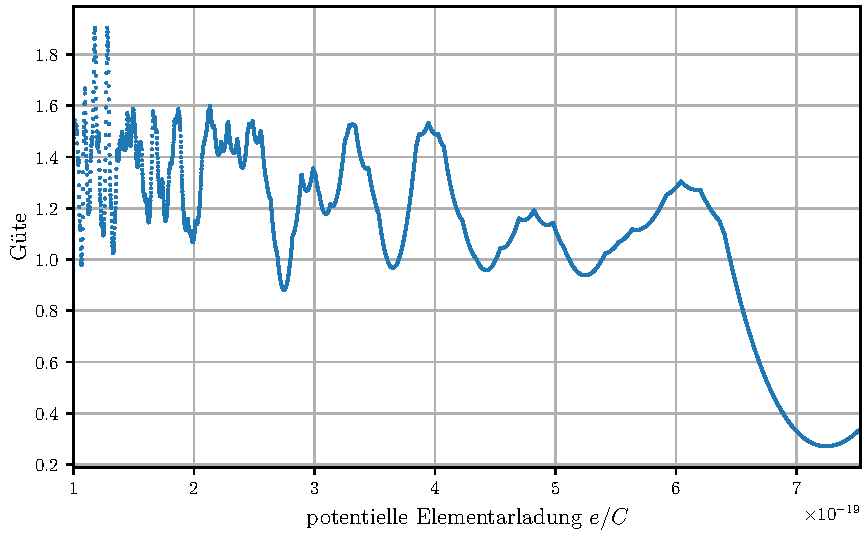
\includegraphics{Guetefunktion.pdf}
  \caption{Gütefunktion gewählter Elementarladungen.}
  \label{fig:Guete}
\end{figure}